\let\nofiles\relax
\documentclass[margin,line]{res}
\usepackage{multirow}
\usepackage{graphicx}
\usepackage{float}
\usepackage{amsmath}
\usepackage{cases}
\usepackage{amsfonts}
\usepackage{stfloats}
\usepackage{cite}
\usepackage{color}
\usepackage{mathrsfs}
\usepackage{animate}
\usepackage{tikz}
\usepackage{longtable}
\usepackage{makecell}
\usetikzlibrary{positioning}

\oddsidemargin -.5in
\evensidemargin -.5in
\textwidth=6.0in
\itemsep=0in
\parsep=0in
% if using pdflatex:
\setlength{\pdfpagewidth}{\paperwidth}
\setlength{\pdfpageheight}{\paperheight} 

\newenvironment{list1}{
  \begin{list}{\ding{113}}{%
      \setlength{\itemsep}{0in}
      \setlength{\parsep}{0in} \setlength{\parskip}{0in}
      \setlength{\topsep}{0in} \setlength{\partopsep}{0in} 
      \setlength{\leftmargin}{0.17in}}}{\end{list}}
\newenvironment{list2}{
  \begin{list}{$\bullet$}{%
      \setlength{\itemsep}{0in}
      \setlength{\parsep}{0in} \setlength{\parskip}{0in}
      \setlength{\topsep}{0in} \setlength{\partopsep}{0in} 
      \setlength{\leftmargin}{0.2in}}}{\end{list}}

\newcommand*{\dif}{\mathop{}\!\mathrm{d}}
\newcommand*{\tabbox}[1]{\Gape[2.2pt]{#1}}
\newcommand*{\ftarrow}{\stackrel{\mathscr{F}}{\longleftrightarrow}}
\newcommand*{\ftfunc}{{\mathscr{F}_f}}
\begin{document}

\name{Course Project for Signal and System  \vspace*{.1in}$\ \ \ \ \ \ \ \ \ \ \ \ \ \ \ \ \ \ \ \ \ \ \ \ \ \ \ \ \ \ \ \ \ \ \ \ \ \ \ \ \ \ \ \ \ \ \ \ \ \ $
\includegraphics[height=6em]{244}}


\begin{resume}
%\section{\sc Contact Information}
\vspace{.05in}
\begin{tabular}{@{}p{3.7in}p{4in}}           
	School of Communication and Information System,  & {\it Name:}  YanSheng Zhu \\         
	Xi'an University of Post and Telecommunications & {\it Identifier:}  05202009
\end{tabular}

\section{\sc I. Where the story begins}
\subsection{\sc \textbf{Some Real Questions}}
When we play the piano,we can press a key, such as Do. Its waveform is like the second curve in the Figure 1. Also we can get La which like the first curve in Figure 1. Then we press these two keys at the same time. Then we will get the third curve in the Figure 1.\par
But when we get a signal which like the third curve, we want to know which two buttons generate it. We want to know how to build this signal.\par
Generally we want to decompose a signal, which like the 4th curve in the Figure 1, into the combination of some simple signal.\par
\begin{figure}[H]
  \begin{minipage}{0.42\linewidth}
    \centerline{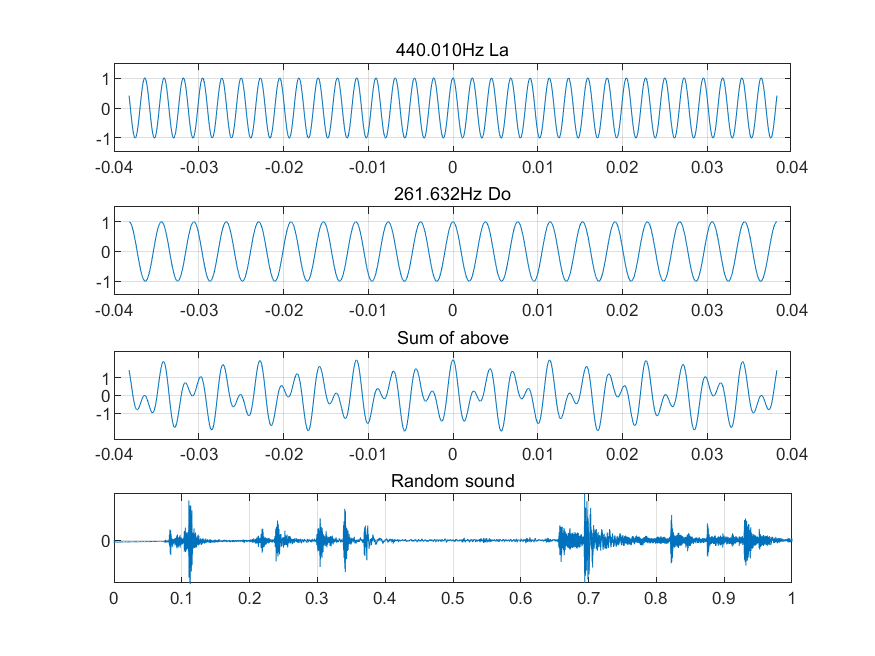
\includegraphics[width=0.9\textwidth]{figure/fig_1.png}}
    \centerline{\textbf{Figure 1}}
  \end{minipage}
  \begin{minipage}{0.55\linewidth}
    \centerline{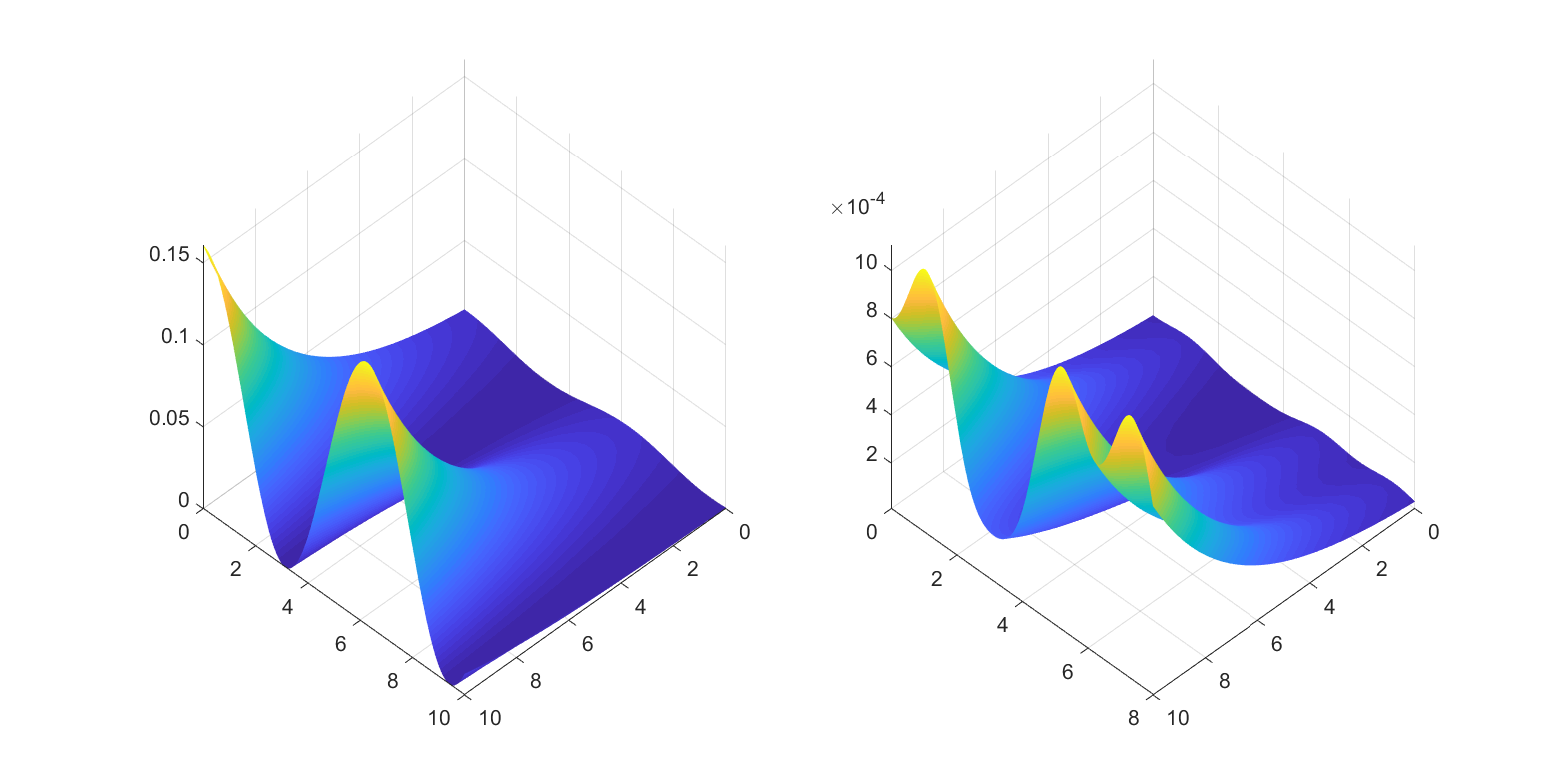
\includegraphics[width=\textwidth]{figure/fig_2.png}}
    \centerline{\textbf{Figure 2}}
  \end{minipage}
\end{figure}
In fact, many physical problems have the same properties, such as heat transfer problem. If we have a rod, which temperature function is $T=cos(x)$ .
The change of its temperature with time t presents a simple exponential decay form, as I showed in the first sub-graph of Figure 2.\par
But for a more complex temperature function $T=f(x)$ like the second sub-graph of Figure 2, if we can decompose it into the composition of a series sine and cosine function, we can simply migrate it to $T=F(x,t)$.

\subsection{\sc \textbf{Intuitive Understanding}}

Let's start with simple one:a sinusoidal signal of 4 beats per second. We can construct a rotating vector whose length is the same as this sinusoidal signal value of the current time. The graph of this vector will like the second sub-graph in Figure 3. We can find a magic phenomenon.When the frequency of this rotating vector is equal to this sinusoidal signal's frequency, a large number of points in this image are biased to the same side.\par
If we imagine this graph is having some kind of mass to it, like metal wire. We can find, as we change the frequency, the center of mass wobbles around a bit at origin. But when the frequency is equal to our signal frequency, the mass center is unusually far to the right. If we draw the x position of the mass center changed by the frequency into a $f-x$ graph. It will be like the third sub-figure in Figure 3. There is a high peak at 4 Hz position.\par
\begin{figure}[H]
	\begin{minipage}{0.48\linewidth}
		\centerline{\animategraphics[autoplay,loop,width=0.8\textwidth]{30}{figure/fig_3/fig-}{1}{601}}
		\centerline{\textbf{Figure 3}}
	\end{minipage}
	\begin{minipage}{0.48\linewidth}
		\centerline{\animategraphics[autoplay,loop,width=0.8\textwidth]{30}{figure/fig_4/fig-}{1}{601}}
		\centerline{\textbf{Figure 4}}
	\end{minipage}
\end{figure}
And we can do the same operation in a combination of two signal: $cos(2\pi 3t)+cos(2\pi 5t)$. Then we can get similar result: two peaks at 3 and 5 Hz. And now, we can make a bold assumptions that we can use the combination of sine or cosine signal to build another arbitrary signal. And we should proof it.

\subsection{\sc \textbf{Proof It!}}

Let us assume $f(t)=\sum\limits^{N}A_n \sin (n\omega t+\phi)$, then we will prove it.
Since we want to using the combination of sine function, we let $f_T(t)$ equals to the sum of n-terms sine signal.
%%Orignal sine formula
$$
f_T(t)=C_0+\sum\limits_{n=1}^N{\sin(n\Omega t+\phi_{n} ) } \quad \Omega=\frac{2\pi}{t}
$$

And we can make some modifications to the formula.
%%Expansion of last formula
$$
f_T(t)=C_0+\sum\limits_{n=1}^N{[
	A_n\sin(n\Omega t)\cos\phi_n+
	A_n\cos(n\Omega t)\sin\phi_n
	]}
$$

Let's denote $a_n=A_n\cos\phi_n$ and $b_n=A_n\sin\phi_n$
%%Denote an and bn
$$
f_T(t)=C_0+\sum\limits_{n=1}^N{[
	a_n\sin(n\Omega t)+
	b_n\cos(n\Omega t)
	]}
$$

Apply Euler's formula
%%Euler's formula
\begin{align}\nonumber
\sin(x)=\frac{e^{jx}-e^{-jx}}{2j}\nonumber \\
\cos(x)=\frac{e^{jx}+e^{-jx}}{2}\nonumber \\
e^{jx}=\cos(x)+j\sin(x)\nonumber
\end{align}
%%Applied euler's formula and merge congeners 
\begin{align}
f_T(t)&=C_0+\sum\limits_{n=1}^{N}{[
	a_n( \frac{ e^{jn\Omega t} + e^{-jn\Omega t} }{2j} )+
	b_n( \frac{ e^{jn\Omega t} + e^{-jn\Omega t} }{2} )
	]}\nonumber \\ 
&=C_0+\sum\limits_{n=1}^{N}{[
	( \frac{b_n-ja_n}{2} )e^{jn\Omega t}+
	( \frac{b_n+ja_n}{2} )e^{-jn\Omega t} 
	]}\nonumber
\end{align}

Then we can denote $C_n=\frac{b_n-ja_n}{2}$ and $C_{-n}=\frac{b_n+ja_n}{2}$
%%Denote Cn
\begin{align}
f_T(t)&=C_0+\sum\limits_{n=1}^{N}{(
	C_n e^{jn\Omega t} + C_{-n} e^{-jn\Omega t}
	)}\nonumber \\
&=\sum\limits_{n=-N}^{N}{C_n e^{jn\Omega t}}\nonumber
\end{align}

Now we have the Fourier series of periodic signal $f_T(t)$, but we don't know how to calculate $C_n$.At this time, we can extract one term from n terms sum.We can denote it as $C_m$.
%%How to calc Cn
\begin{flalign}
&f_T(t)=C_m e^{jm\Omega t} + 
	\sum\limits_{ \substack{n=-N \\ n\neq m} }^{N}{C_n e^{jn\Omega t}} \nonumber \\
&C_m e^{jm\Omega t}=f_T(t)-
	\sum\limits_{ \substack{n=-N \\ n\neq m} }^{N}{C_n e^{jn\Omega t}} \nonumber \\
&C_m=f_T(t) e^{-jm\Omega t}-
	\sum\limits_{ \substack{n=-N \\ n\neq m} }^{N}{C_n e^{j(n-m)\Omega t}} \nonumber
\end{flalign}

We can do integration in both sides
%%Integration of left and right
\begin{align}
&\int_{0}^{T}{C_m\dif t}=\int_{0}^{T}{(f_T(t) e^{-jm\Omega t}-
	\sum\limits_{ \substack{n=-N \\ n\neq m} }^{N}{C_n e^{j(n-m)\Omega t}})
	\dif t} \nonumber \\
&TC_m=\int_{0}^{T}{[f_T(t) e^{-jm\Omega t}-
	\sum\limits_{ \substack{n=-N \\ n\neq m} }^{N}{C_n e^{j(n-m)\Omega t}}]
	\dif t} \nonumber
\end{align}

Since integration and summation is linear operation, we can put integration into summation.
%%Swap integratuion and summation
\begin{align}
	&TC_m=\int_{0}^{T}{f_T(t) e^{-jm\Omega t}} \dif t -
		\sum\limits_{ \substack{n=-N \\ n\neq m} }^{N}{
			\int_{0}^{T}C_n e^{j(n-m)\Omega t} \dif t
		} \nonumber
\end{align}

For the inner item of summation, we have
%%Calculate orthogonal terms 
\begin{align}
&\int_{0}^{T}{C_n e^{j(n-m)\Omega t} \dif t } \nonumber \\
=&\ C_n\int_{0}^{T} e^{j(n-m)\Omega t} \nonumber \\
=&\ \frac{C_n}{j(n-m)\Omega} \Big[ e^{ j(n-m) \frac{2\pi}{T} t} \Big]_{0}^{T} \nonumber \\
=&\ 0 \nonumber
\end{align}

So, we can get
%%Cn result
$$
C_n=\frac{1}{T}\int_0^T{f_T(t) e^{-jn\Omega t} \dif t}
$$

\subsection{\sc \textbf{Is That True?}}

Now, we can get a series which is contain the combination of sine and cosine function. We can simply use it to verify our suggestion. If we have a square wave with frequency of 1Hz and 50\% duty cycle. Let's calculate its Fourier coefficient. And we should always start with $C_0$.
%%C0 of square wave
\begin{align}
C_0 &= \ \int_{0}^{1}{f_T(t) e^{-j\Omega t \cdot 0} \dif t} \quad \Omega=\frac{2\pi}{T} \nonumber \\
	&=\ \int_{0}^{1}{f_T(t) \dif t} \nonumber \\
	&=\ \int_{0}^{0.5}{\dif t} + \int_{0.5}^{1}{- \dif t} \nonumber \\
	&=\ 0 \nonumber \\
C_n &= \ \int_{0}^{1}{ f_T(t) e^{-jn\Omega t} \dif t} \nonumber \\
	&= \ \int_{0}^{0.5}{e^{-jn\Omega t} \dif t} +
		 \int_{0.5}^{1}{-e^{-jn\Omega t} \dif t} \nonumber \\
	&= \ \Big[-\frac{1}{jn\Omega} e^{-jn\Omega t}\Big|_{0}^{0.5} \Big] -
	   	 \Big[\frac{1}{jn\Omega} e^{-jn\Omega t}\Big|_{0.5}^{1} \Big] \nonumber
\end{align}
Apply $\Omega \ = \ \frac{2\pi}{T} $
\begin{align}
C_n	&= \ \Big[-\frac{1}{jn2\pi} e^{-jn2\pi t}\Big|_{0}^{0.5} \Big] -
		 \Big[\frac{1}{jn2\pi} e^{-jn2\pi t}\Big|_{0.5}^{1} \Big] \nonumber \\
	&= \ \cfrac{j}{2\pi n}\Big[ e^{-j\pi n} -1 -e^{-j2\pi n} +e^{-j\pi n} \Big] \nonumber \\
	&= \ \cfrac{j}{2\pi n}\Big[ 2e^{-j\pi n -1 -e^{-j2\pi n}} \Big] \nonumber
\end{align}
We can simply calculate that $e^{-j2\pi n}=1$ and $e^{-j\pi n}=(-1)^{n}$. So we can get
\begin{align}
C_n &= \ \cfrac{j}{\pi n}\Big[ (-1)^n-1 \Big] \nonumber \\
	&=\begin{cases}
		\cfrac{-2j}{\pi n}&  {odd \ n} \\
		0&  {even \ n}
 	  \end{cases}	\nonumber
\end{align}
And the Fourier series of square wave will be
$$
\mathscr{F}_f(t)= \ \cfrac{4}{\pi} \sum\limits_{k=1}^K{\cfrac{1}{2k-1} \sin [2\pi (2k+1)t]}
$$
Using Matlab to verify it.
\begin{figure}[H]
	\centerline{\animategraphics[autoplay,loop,scale=0.5]{1}{figure/fig_5/fig-}{0}{5}}
\end{figure}
\clearpage

\section{\sc II. When the infinite sum has to be applied}
\subsection{\sc \textbf{Apply Infinity Summation}}
Now, we have an almost-Fourier series. But we can find ,when we use sine wave to build square wave, this sequence converges to the square wave except at the point $x_0 = 0$, which a point of discontinuity of it.There has been a dispute in the field of mathematics about whether sinusoids can be combined into a signal with edges and corners. The protagonists of this dispute are Fourier and Lagrange. \par
Because of the finite sum of sinusoids satisfies infinitely smooth condition, infinitely summation of sinusoids must be applied in order to build signal which has sharp edge. It looks like 
$$
f_T(t) = \sum\limits_{n=-\infty}^{\infty} {C_n e^{jn\Omega t}}
$$
When the infinite sum has to be applied, we should check its convergence.Fourier claims that any arbitrary periodic signal can be expand in its Fourier series. No one can prove or falsify it until Dirichlet did the proof. \par

\begin{itemize}
\item Continuous case: If the periodic signal $f(t)$ is a continuous function of t, then its Fourier series converge uniformly.
$$
\lim_{N \rightarrow \infty} \left[ f(t) - \sum\limits_{n=-N}^{N}{C_n e^{jn\Omega t}} \right] = 0
$$
\item Finite-energy case: If periodic signal $f(t)$ has finite energy in a single period, the Fourier series converge in the MSE sense.
$$
\lim_{N \rightarrow \infty} \cfrac{1}{T} \int_{T}\left| f_T(t) - \sum\limits_{n=-N}^{N}C_n e^{-jn\Omega t} \right| \dif t  = 0\nonumber
$$
\item Dirichlet case:
\begin{enumerate}
	\item Over a single period, $f(t)$ is absolutely integrable (i.e.,$\int_{T}\left| f(t) \right| < \infty$)
	\item In any finite interval of time $f(t)$ is of bounded variation. In other words, there must be a finite number of maxima and minima in a single period of $f(t)$
	\item In any finite interval of time, $f(t)$ has a finite number of discontinuities, each of which is finite.
\end{enumerate}
If $f(t)$ is a periodic signal satisfying the Dirichlet conditions, and $t_a$ is the discontinuities of $f(t)$, then:
\begin{enumerate}
	\item For $t \neq t_a$
	$$
	\lim_{N \rightarrow \infty} \left[ f(t) - \sum\limits_{n=-N}^{N} C_n e^{jn\Omega t} \right] = 0 \quad t \neq t_a
	$$
	\item For $t = t_a$
	$$
	\lim_{N \rightarrow \infty} \left[ \sum\limits_{n=-N}{N} C_n e^{jn\Omega t_a}\right] =
	\frac{1}{2}\left[ f(t_a^{-} + f(t_a^{+})) \right]
	$$
\end{enumerate}
\textbf{Proof:} \\
We need some result which have been proofed to help us proof this one.\\
Result 1(Riemann-Lebesgue's Theory): If $f(x)$ and $f^{'}(x)$ are piecewise continuous on $\left[ a,b \right]$, then
\begin{align}
\lim_{\lambda \rightarrow \infty} \int_{a}^{b} f(x)\sin(\lambda x) \dif x = 0 \nonumber \\
\lim_{\lambda \rightarrow \infty} \int_{a}^{b} f(x)\cos(\lambda x) \dif x = 0 \nonumber
\end{align}
Result 2(Fourier partial sums): We have 
\begin{align}
	D_N(\alpha) &= \cfrac{\sin(N+\frac{1}{2})\alpha}{2\pi sin(\frac{\alpha}{2})} \nonumber \\
	f_N(x) &=\frac{1}{\pi}\int_{-\pi}^{\pi}{f(t)D_N(t-x)} \dif t \nonumber
\end{align}
The $f_N(x)$ is called the \textbf{Fourier partial sums}. And the Dirichlet Kernel is defined by
\begin{align}
	D_N(x) = 
	\begin{cases}
		\cfrac{ \sin\left[ (N+\cfrac{1}{2})x \right] }{2\pi \sin(\frac{x}{2})} & x \neq 0,\pm 2\pi \cdots \\
		\cfrac{2N+1}{2\pi} & x=0,\pm 2\pi, \cdots
	\end{cases} \nonumber
\end{align}
And, we can get 
$$
\int_{-\pi}^{0} D_N(x) \dif x = 
\int_{0}^{\pi} D_N(x) \dif x =
\cfrac{1}{2}
$$
Without loss of generality, we can assume that $f(x)$ is defined and $2\pi$-periodic on the $\mathbb{R}$.So, the function $D_N(x)f(t)$ is $2\pi$-periodic in t.
Using the Dirichlet Kernel, we obtain
$$
f_N(x) = \int_{-\pi}^{pi} f(t) D_N(t-x) \dif t
$$
denote $u=t-x$,
\begin{align}
f_N(x) 	&= \ \int_{-\pi -x}^{\pi -x} f(u+x) D_N(u) \dif u \nonumber \\
	 	&= \ \int_{-\pi}^{\pi} f(u+x) D_N(u) \dif u \label{XX}
\end{align}
Since $D_N(x)$ is a even function, so
\begin{align}
f_N(x) = \ \int_{-\pi}^{\pi} f(x-u) D_N(u) \dif u \label{YY}
\end{align}
Then, calculate the arithmetic mean of \eqref{XX} and \eqref{YY}
$$
f_N(x)=\int_{-\pi}^{\pi}\cfrac{f(x+u)+f(x-u)}{2}D_N(u) \dif u
$$
Since the function inside the integral are even
$$
f_N(x)=\int_{0}^{\pi}\left[ f(x+u)+f(x-u) \right]D_N(u) \dif u
$$
On the other hand, we have
$$
\int_{0}^{\pi}D_N(u) \dif u = \frac{1}{2}
$$
which gives:
$$
\cfrac{f(x^{+})+f(x^{-})}{2} = \int_{0}^{\pi} \left[ f(x^{+})+f(x^{-}) \right]D_N(u) \dif u
$$
Hence
\begin{align}
	\cfrac{f(x^{+})+f(x^{-})}{2} - f_N(x) &=
	\ \int_{0}^{\pi} \left[ \phi_{1}(u,x)+\phi_{2}(u,x) \right] D_N(u) \dif u \nonumber \\
	\phi_{1}(u,x)&=f(x^{+})-f(x+u) \nonumber \\
	\phi_{2}(u,x)&=f(x^{-})-f(x-u) \nonumber
\end{align}
And, we can set $g(u)=\cfrac{\phi_{1}(u)}{u}$, then
$$
U(u)=\cfrac{u}{2 \sin( \frac{u}{2} ) } \ for \ u \neq 0, \ U(0)=1
$$
$U(u)$ is continuous on $\left[-\pi,\pi\right]$, Result 1 will imply
$$
\lim_{N \rightarrow \infty}\int_{0}^{\pi}g(u)U(u)sin(N+\frac{1}{2})u \dif u = 0
$$
And since $\int_{0}^{\pi}g(u)U(u)sin(N+\frac{1}{2})u \dif u = \int_{0}^{\pi}\phi_{1}(u,x)D_N(u)\dif u$, we can get
$$
\int_{0}^{\pi} \phi_{1}(u,x)D_N(u)\dif u = 0
$$
The proof of 
$$
\lim_{N \rightarrow \infty}\int_{0}^{\pi}\phi_{2}(u,x)\dif u=0
$$
will be done similarly.
So we can obtain 
\begin{align}
	& \cfrac{f(x^{+})+f(x^{-})}{2}-f_N(x)=0 \quad (N \rightarrow \infty) \nonumber \\
	& f_N(x)=\cfrac{f(x^{+})+f(x^{-})}{2} \quad (N \rightarrow \infty) \nonumber
\end{align}
\end{itemize}
Although many signal satisfy the Dirichlet conditions, not all signals satisfy these conditions.
\begin{figure}[H]
	\centerline{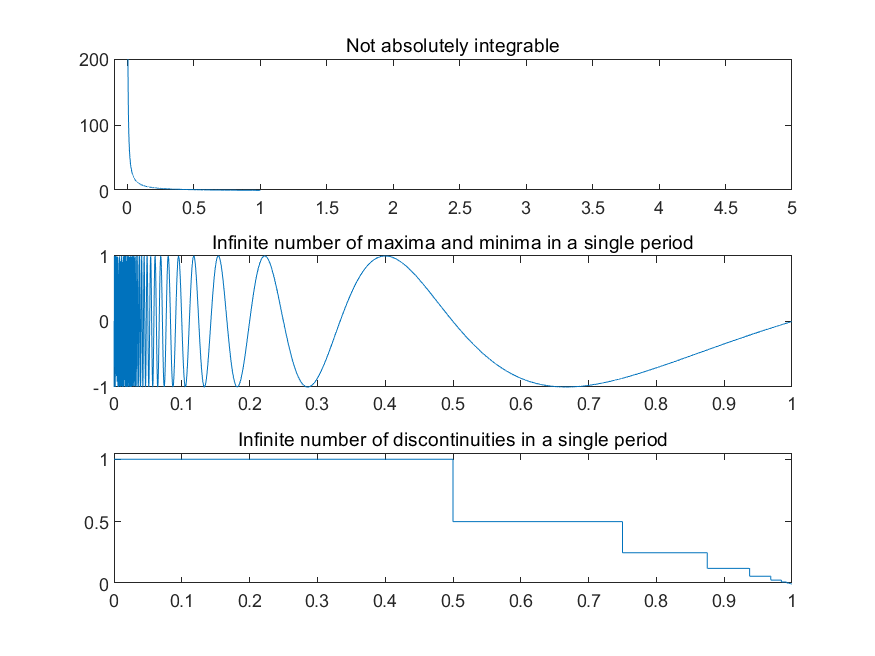
\includegraphics[width=0.55\linewidth]{figure/fig_6.png}}
\end{figure}
\subsection{\sc \textbf{Gibbs Phenomenon}}
In 1898, American Albert Michelson made a harmonic analyzer. When he tested the square wave, he was surprised to find that the $X_n(T)$ of the square wave jumped near the discontinuous points, and the peak size of the fluctuation did not seem to decrease with the increase of n! So he wrote to Gibbs, the famous mathematical physicist at that time. Gibbs got interested to the behavior of the sequence of Fourier partial sums around these points. \par
Indeed, when x is close to the point 0, the graphs present a bump, even when N is quite large. Let us do some calculations to justify this phenomenon. Consider the derivative of $\mathscr{F}_f(t)$.
\begin{align}
\mathscr{F}^{'}_f(t) 
	&= \ \cfrac{4}{\pi} \sum\limits_{n=0}^N{\cos [2\pi (2k+1)t]} \nonumber \\
	&= \ \cfrac{4}{\pi} \left[ \cos(t) + \cos(3t) + cos(5t) + \cdots + cos((2N-1)t) \right] \nonumber 
\end{align}
Using trigonometric identities, we get 
\begin{align}
\pi\sin(t) \mathscr{F}^{'}_f(t) 
	&= \ 2\left\{ \sin(2t) + \left[\sin(4t)-\sin(2t)\right] + \left[\sin(6t)-\sin(4t)\right] + \cdots + \left[ \sin(2nt)-\sin(2n-2)t \right] \right\} \nonumber \\
	&= \ 2\sin(2nt) \nonumber
\end{align}
So the critical points of $\mathscr{F}_f(t)$ are 
$$
2nt = \pm\pi , \pm 2\pi,\cdots,\pm (2n-1)\pi
$$
Since the functions are odd, we will only focus on the behavior to the right of 0. The closest critical point to the right of 0 is $\frac{\pi}{2n}$. Hence 
$$
\mathscr{F}_f(\cfrac{\pi}{2n}) = \cfrac{4}{\pi} {
	\sin(\frac{\pi}{2n}) + \cfrac{\sin(\frac{3\pi}{2n})}{3} + \cdots +
	\cfrac{\sin(\frac{(2n-1)\pi}{2n})}{2n-1}
}
$$
In order to find the asymptotic behavior of the this sequence, when n is large, we will use the Riemann sums. Indeed, consider the function $Sa(t) = \frac{\sin(t)}{t}$ on the interval $[0,\pi]$, and the partition $\left\{{\frac{k\pi}{n}}, \;\;k \in [1,n]\right\}$ of $[0,\pi]$. So the Riemann sums
$$
\frac{\pi}{n}
\left(
	\cfrac{\sin(\cfrac{\pi}{2n})}{\cfrac{\pi}{2n}} + \cdots +
	\cfrac{\sin(\cfrac{(2n-1)\pi}{2n})}{\cfrac{(2n-1)\pi}{2n}}
\right)
$$
converges to $\int_{0}^{\pi} Sa(t) \dif t$. Easy calculations show that these sums are equal to 
$$
\cfrac{\pi}{2}{\mathscr{F}_f \left( \cfrac{\pi}{2n} \right) }
$$

Hence

$$
\lim_{n \rightarrow \infty} \mathscr{F}_f \left(\frac{\pi}{2n}\right) = \frac{2}{\pi}\int_{0}^{\pi}Sa(t) \dif t.
$$

Using Taylor polynomials of $\sin(t)$ at 0, we get

$$
\frac{2}{\pi}\int_{0}^{\pi}\frac{\sin(t)}{t} \dif t = 2 - \frac{\pi^2}{9} + \frac{\pi^4}{300} - \frac{\pi^6}{17640}+\ldots
$$

i.e. up to two decimals, we have

$$
\frac{2}{\pi}\int_{0}^{\pi}\frac{\sin(t)}{t} \dif t = 1.18
$$
These bumps seen around 0 are behaving like a wave with a height equal to 0.9045. This is not the case only for this function. Indeed, Gibbs showed that if f(t) is piecewise smooth on $[-\pi,\pi]$, and $t_0$ is a point of discontinuity, then the Fourier partial sums will exhibit the same behavior, with the bump's height almost equal to 
$$
0.09\left[ f(t_0+) + f(t_0-)\right]
$$
This is called \textbf{Gibbs Phenomenon}: Even though $N \rightarrow \infty$, there is approximately $9\%$ difference at the discontinuity.
\begin{figure}[H]
	\centerline{\textbf{Square wave's Gibbs phenomenon near $x=0$}}
	\centerline{\animategraphics[autoplay,loop,scale=0.5]{2}{figure/fig_7/fig-}{1}{10}}
\end{figure}
\clearpage

\section{\sc III. Open the gate to frequency domain}
\hspace{.05in}
\subsection{\sc \textbf{Build up a Periodic Signal}}
Fourier series is actually signal construction.
\begin{itemize}
	\item \textbf{Select building blocks:} choose frequency components whose frequency is the integer multiples of the signal frequency.
	\item \textbf{Polish building blocks:} using Fourier coefficients to modify the amplitude and phase of blocks.
	\item \textbf{Build your signal up:} achieved by the linear combination of modified building block.
\end{itemize}
\begin{figure}[H]
	\begin{minipage}{0.5\linewidth}
		\centerline{\animategraphics[autoplay,loop,width=0.8\linewidth]{10}{figure/fig_8/fig-}{0}{199}}
	\end{minipage}
	\begin{minipage}{0.5\linewidth}
		\centerline{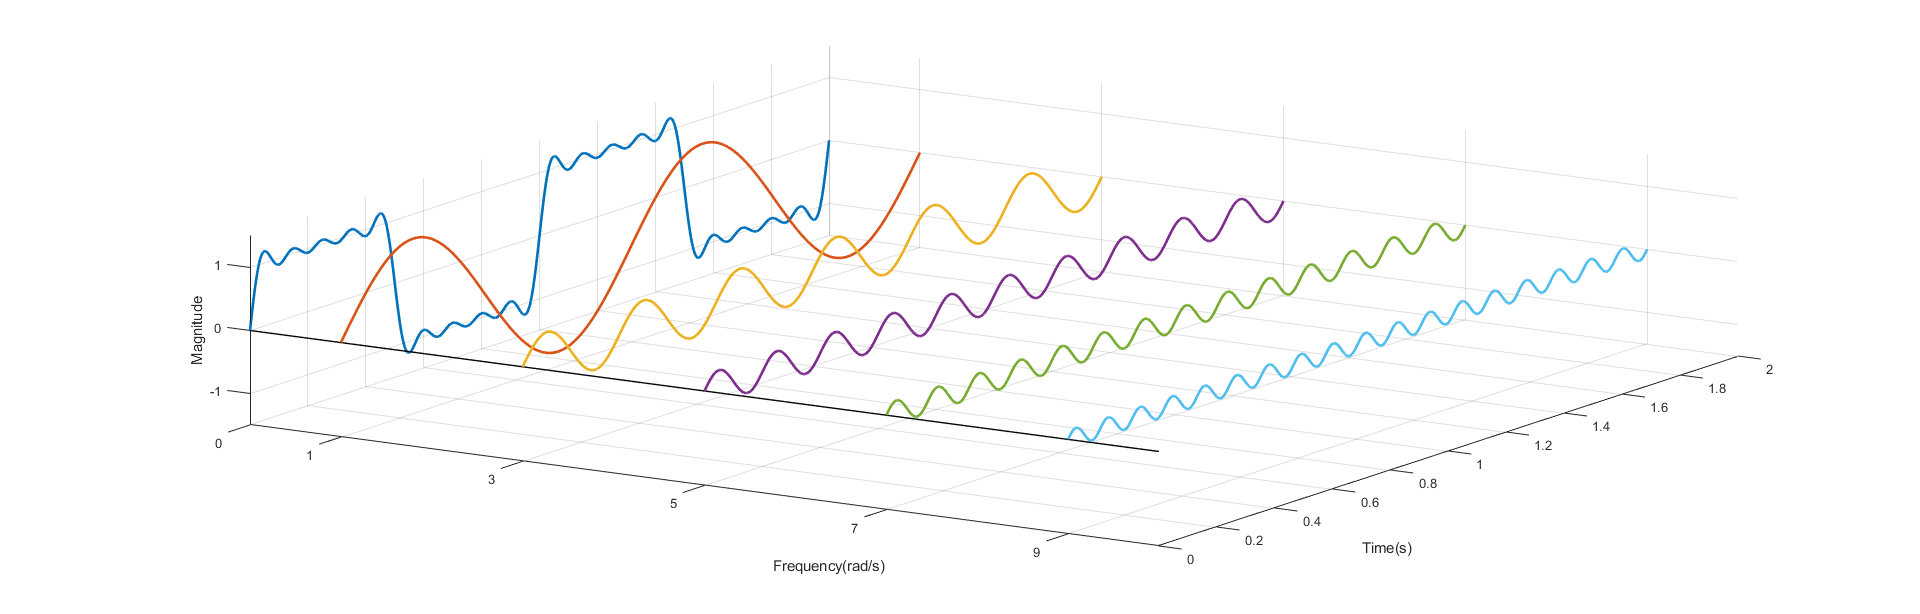
\includegraphics[width=0.9\textwidth]{figure/fig_9.png}}
	\end{minipage}
\end{figure}
\subsection{\sc \textbf{Signal Spectrum}}
And based on Fourier series, any arbitrary periodic signal $f(t)$ of period $T$ can be decomposed by linear combination of sinusoidals.
\begin{align}
f(t)	&= \ \frac{A_0}{2} + \sum\limits_{n=1}^{\infty}{A_n \cos (n \Omega t + \phi_{n})} \nonumber \\
		&= \ \frac{A_0}{2} + \sum\limits_{n=1}^{\infty}{a_n \cos (n \Omega t)} + \sum\limits_{n=1}^{\infty}{b_n \sin (n \Omega t)} \nonumber \\ 
		&= \ \sum\limits_{n=-\infty}^{\infty}{C_n e^{jn\Omega t} } , \ C_n=\left|C_n\right| e^{j\angle C_n} \nonumber
\end{align}
With the above content, we can no longer focus on the performance of the signal in the time domain, but analyze its performance in the frequency domain. We can characterize a signal by its spectrum. Signal Spectrum characterize how the signal parameters change with frequency components.\par 
\begin{itemize}
	\item \textbf{Magnitude Spectrum:} variation between the magnitude of harmonics and the frequency component.\par 
	\begin{figure}[H]
		\centerline{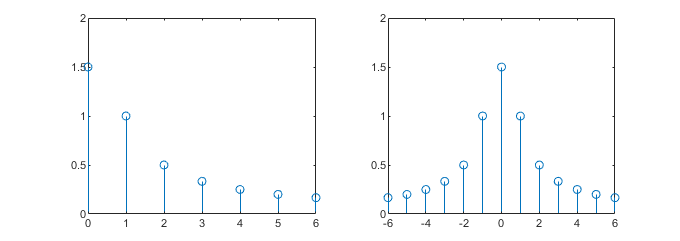
\includegraphics[width=0.9\linewidth]{figure/fig_10.png}}
		\centerline{\textbf{Left:}single-side magnitude spectrum}
		\centerline{\textbf{Right:}double-side magnitude spectrum}
	\end{figure}
	By applying $\left|C_n\right|=\frac{A_n}{2}$, we can get the double-side magnitude spectrum.\par
	\item \textbf{Phase Spectrum:} variation between the phase of harmonics and the frequency component.\par 
	\begin{figure}[H]
		\centerline{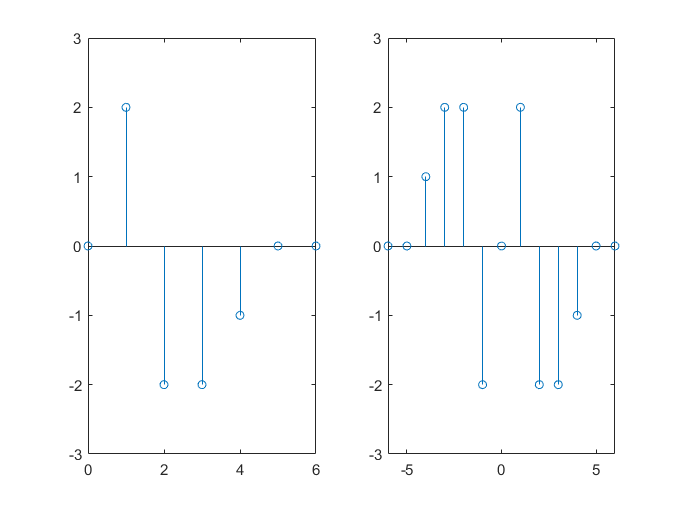
\includegraphics[width=0.9\linewidth]{figure/fig_11.png}}
		\centerline{\textbf{Left:}single-side phase spectrum}
		\centerline{\textbf{Right:}double-side phase spectrum}
	\end{figure}
	By applying $\angle C_n=\phi_n$, we can get the double-side phase spectrum.
\end{itemize}
From the figure above, we can obtain that \textbf{The double-side magnitude spectrum is evenly symmetric while the double-side phase spectrum is oddly symmetric if the periodic signal is real.} 
\subsection{\sc \textbf{Power of Periodic Signal}}
In general, periodic signal is a power signal.
$$
\mathscr{P}=\frac{1}{T} \int_{0}^{T}\left|f(t)\right|^2 \dif t
$$
By applying Fourier series
\begin{align}
\mathscr{P} = \ \frac{1}{T} \int_{0}^{T} {\sum\limits_{n=-\infty}^{\infty} \sum\limits_{m=-\infty}^{\infty} {C_n C_m e^{j(n-m)\Omega t}}} \dif t \nonumber
\end{align}
And we can obtain that
\begin{align}
	\int_{0}^{T} e^{j(n-m)t}=
	\begin{cases}
		T & n=m \\
		0 & n\neq m
	\end{cases} \nonumber
\end{align}
Hence
\begin{align}
	\mathscr{P} 
	&= \ \frac{1}{T} \sum\limits_{n=-\infty}^{\infty} \sum\limits_{m=-\infty}^{\infty} \left|C_n\right| \cdot \left|C_m\right| \cdot T, \ n=m \nonumber \\
	&= \ \sum\limits_{n=-\infty}^{\infty}{\left|C_n\right|^2} \nonumber \\
	&= \ \left(\frac{A_0}{2}\right)^2 + \frac{1}{2}\sum\limits_{n=1}^{\infty}A_n^2 \nonumber
\end{align}
This is called Parseval's Theorem.
\subsection{\sc \textbf{The Relation between Time-Domain and Frequency-Domain}}
\begin{figure}[H]
	\centering
	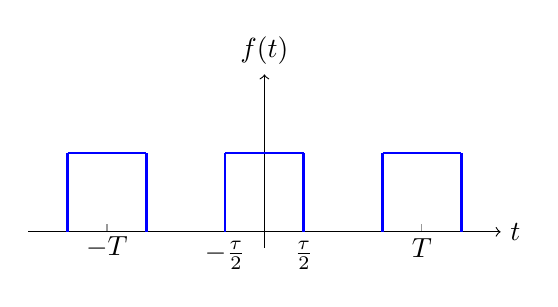
\begin{tikzpicture}
		\draw[gray!80] (-2,0) -- (-2,0.1);
		\draw[gray!80] (2,0) -- (2,0.1);
		\draw[->] (-3,0) -- (3,0) node[right] {$t$};
		\draw[->] (0,-0.2) -- (0,2) node[above] {$f(t)$};
		\draw[blue,line width=1pt] (-2.5,0) -- (-2.5,1);
		\draw[blue,line width=1pt] (-2.5,1) -- (-1.5,1);
		\draw[blue,line width=1pt] (-1.5,1) -- (-1.5,0);
		\draw[blue,line width=1pt] (-0.5,0) -- (-0.5,1);
		\draw[blue,line width=1pt] (-0.5,1) -- (0.5,1);
		\draw[blue,line width=1pt] (0.5,1) -- (0.5,0);
		\draw[blue,line width=1pt] (1.5,0) -- (1.5,1);
		\draw[blue,line width=1pt] (1.5,1) -- (2.5,1);
		\draw[blue,line width=1pt] (2.5,1) -- (2.5,0);
		\node at (-2,-0.2) {$-T$};
		\node at (2,-0.2) {$T$};
		\node at (-0.5,-0.3) {$-\frac{\tau}{2}$};
		\node at (0.5,-0.3) {$\frac{\tau}{2}$};
	\end{tikzpicture} \\
	\centering\textbf{Signal 1}
\end{figure}

If we have a signal which like \textbf{Signal 1}, we can get

\begin{align}
C_n &= \frac{1}{T} \int_{-\frac{T}{2}}^{\frac{T}{2}} f(t) e^{-jn \Omega t} \dif t \nonumber \\
	&= \left. \frac{1}{T} \cfrac{ e^{-j \Omega t} }{ -jn\Omega } \right|_{-\frac{\tau}{2}}^{\frac{\tau}{2}} \nonumber \\
	&= \frac{\tau}{T}Sa(\frac{n\pi \tau}{T}) \nonumber 
\end{align}

Then we can define the signal bandwidth: \\
\textbf{The spectrum bandwidth contains most significant harmonics contributing in signal construction}. \par
So we can obtain that reject harmonics beyond bandwidth does not distort signal severely. Then we can set $\tau$ and $T$ to some unique value. Firstly, we can set $T$ to a constant value $4$, while changing the ratio of $T$ to $\tau$.
\begin{figure}[H]
	\centerline{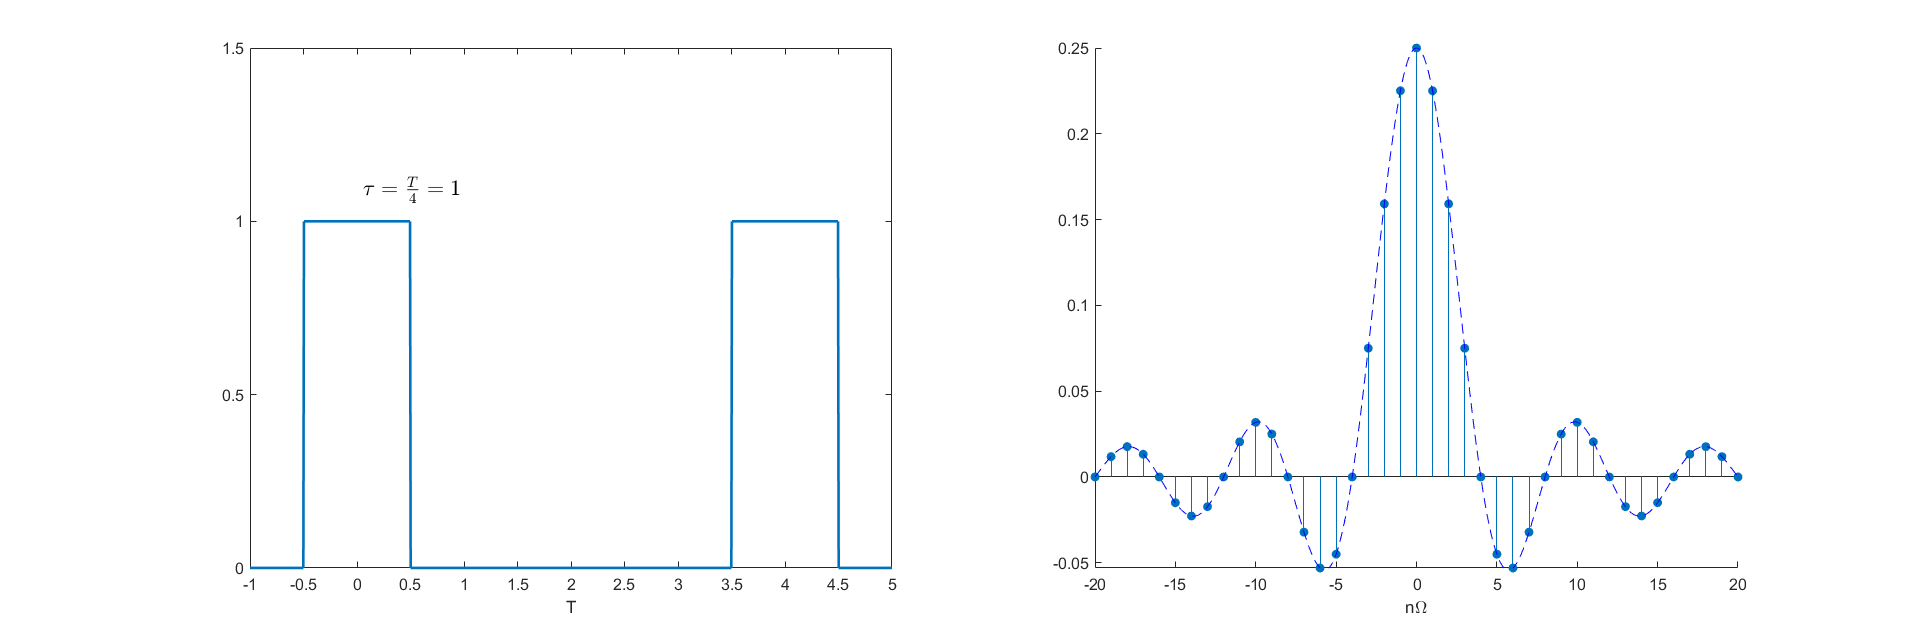
\includegraphics[width=0.9\linewidth]{figure/bw_1.png}}
	\centerline{\textbf{$\tau = \frac{T}{4} = 1$}}
\end{figure}
\begin{figure}[H]
	\centerline{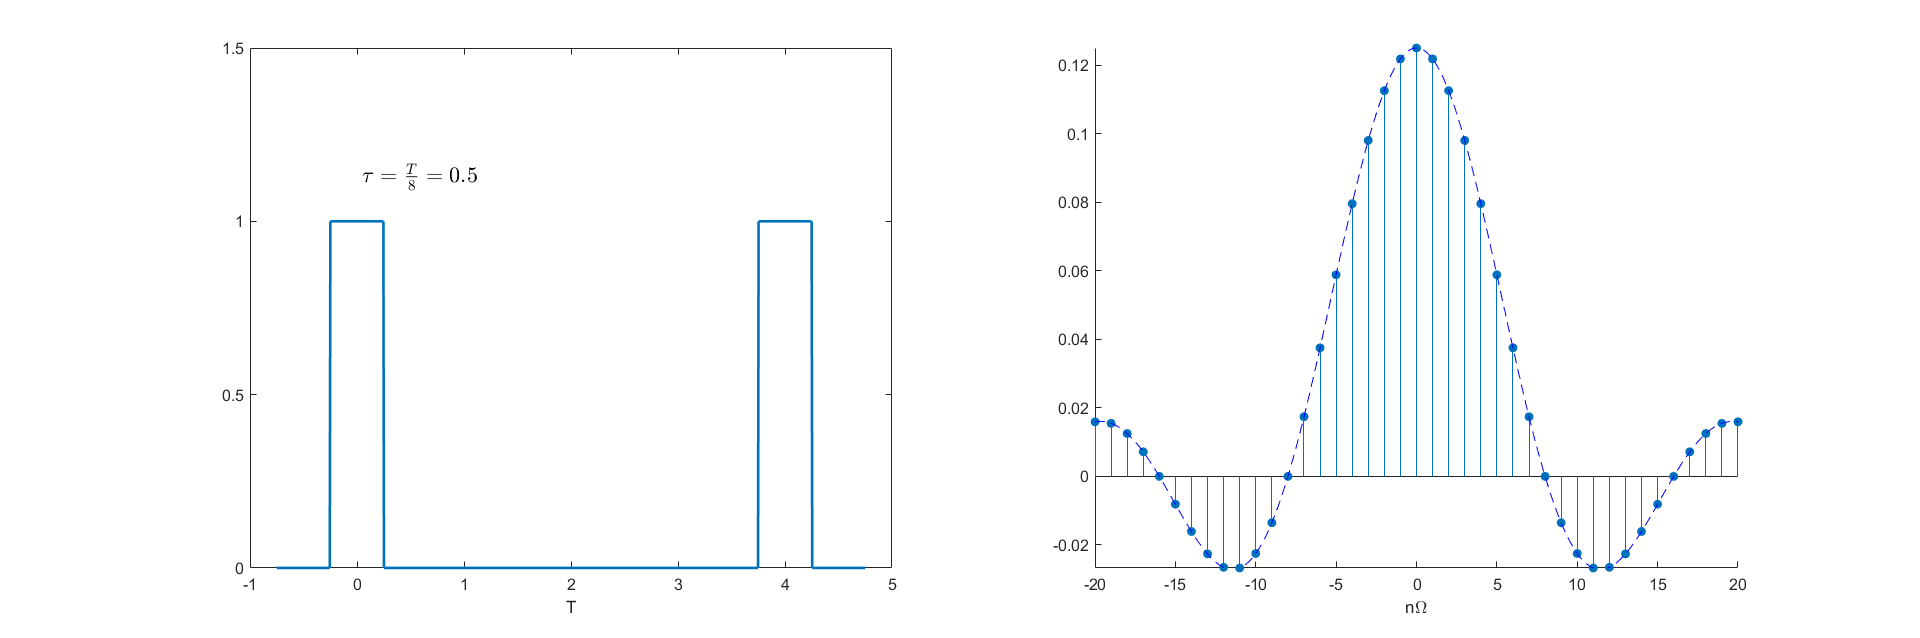
\includegraphics[width=0.9\linewidth]{figure/bw_2.png}}
	\centerline{\textbf{$\tau = \frac{T}{8} = 0.5$}}
\end{figure}
\begin{figure}[H]
	\centerline{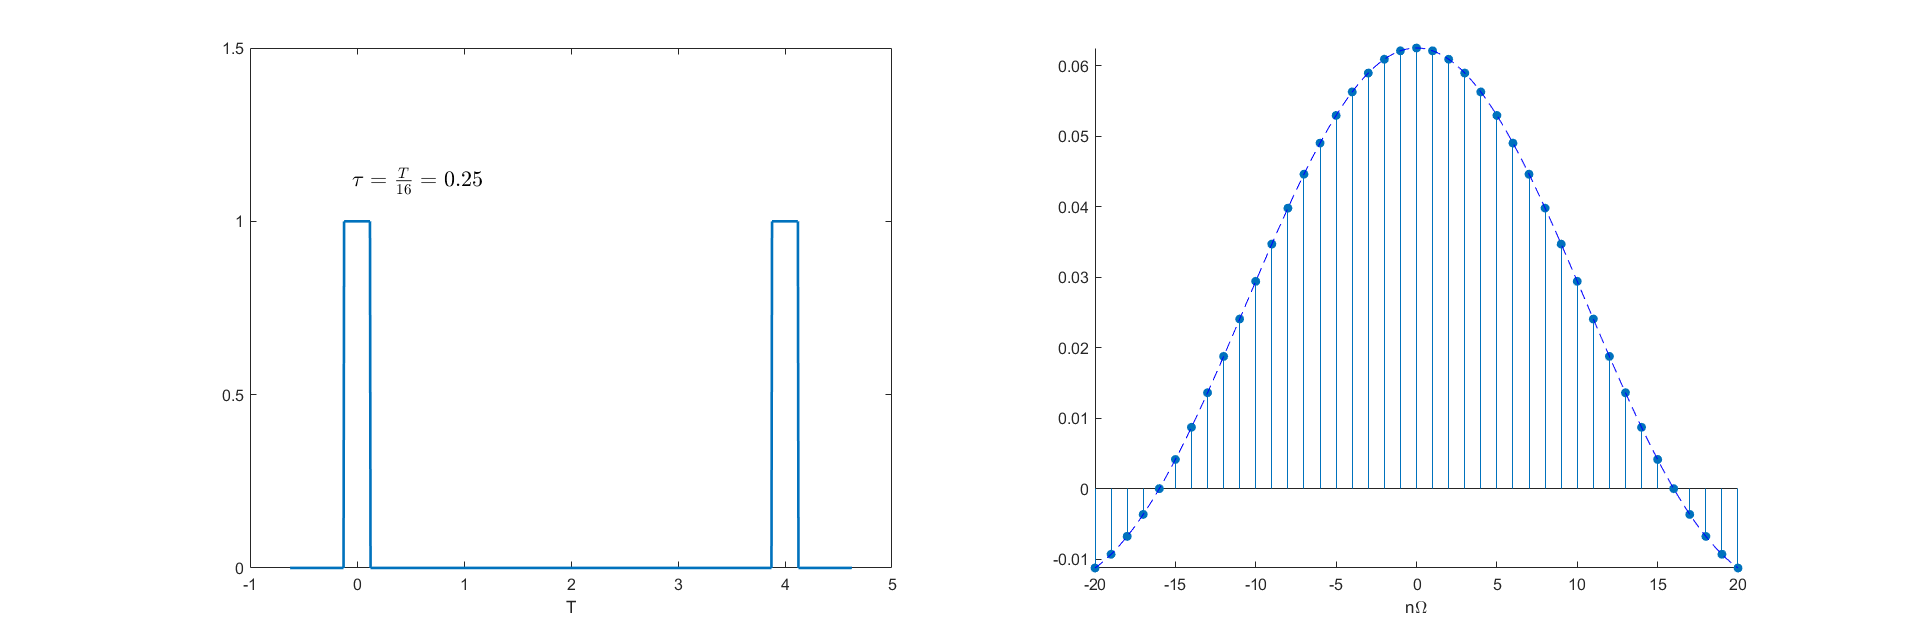
\includegraphics[width=0.9\linewidth]{figure/bw_3.png}}
	\centerline{\textbf{$\tau = \frac{T}{16} = 0.25$}}
\end{figure}
According to the three figures above, we can conclude 
\textbf{the 1st reciprocal relation between time-domain and frequency-domain:} 
The more expand the signal is in time-domain, the more compressed the signal is in frequency-domain. In short, the signal bandwidth is inversely proportional to the time duration of the signal $\tau$.
Also, we can set $\tau$ to a constant value, and change the the ratio of $\tau$ to $T$.
\begin{figure}[H]
	\centerline{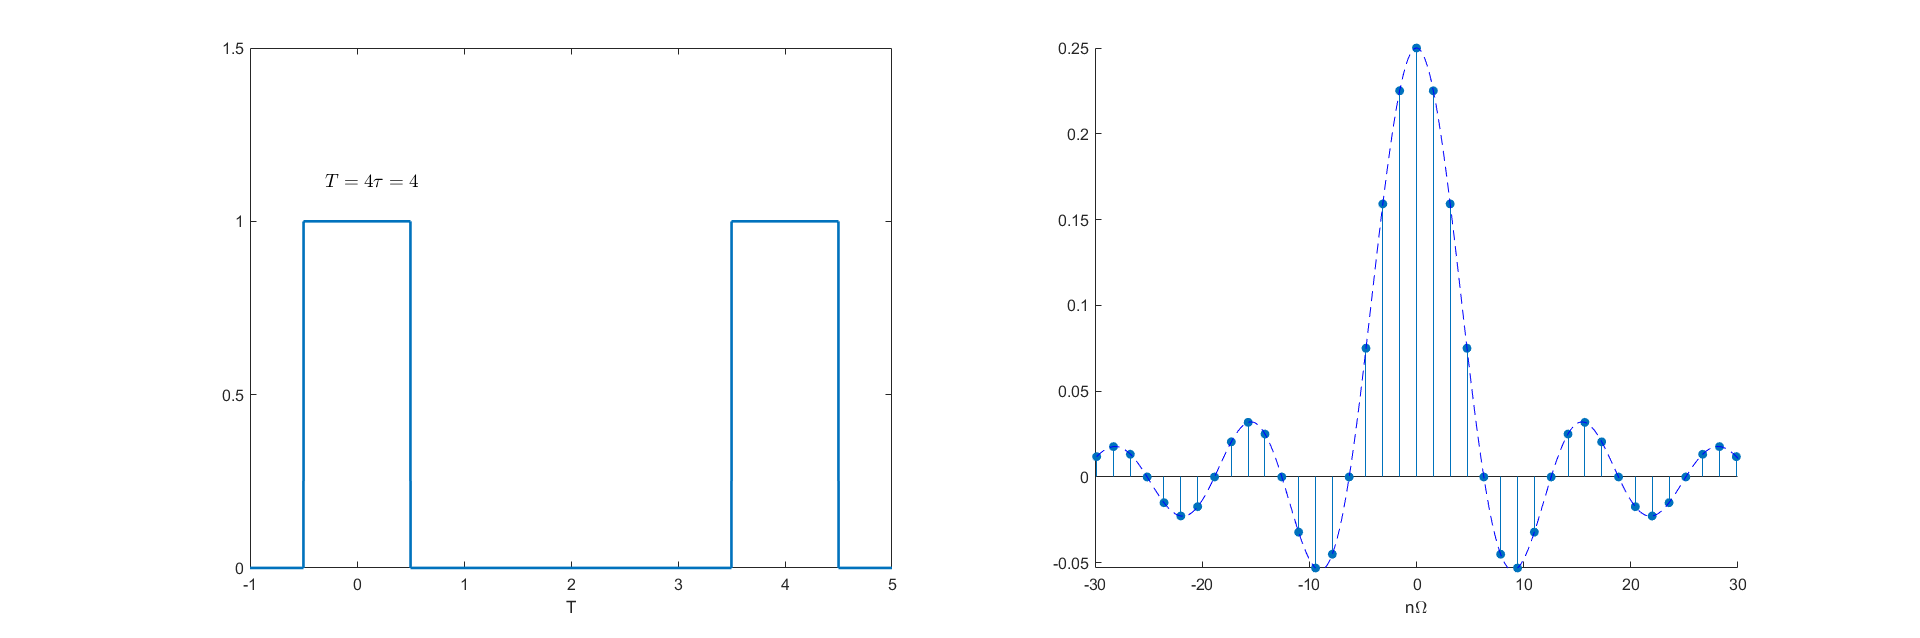
\includegraphics[width=0.9\linewidth]{figure/bw_4.png}}
	\centerline{\textbf{$T = 4\tau = 4$}}
\end{figure}
\begin{figure}[H]
	\centerline{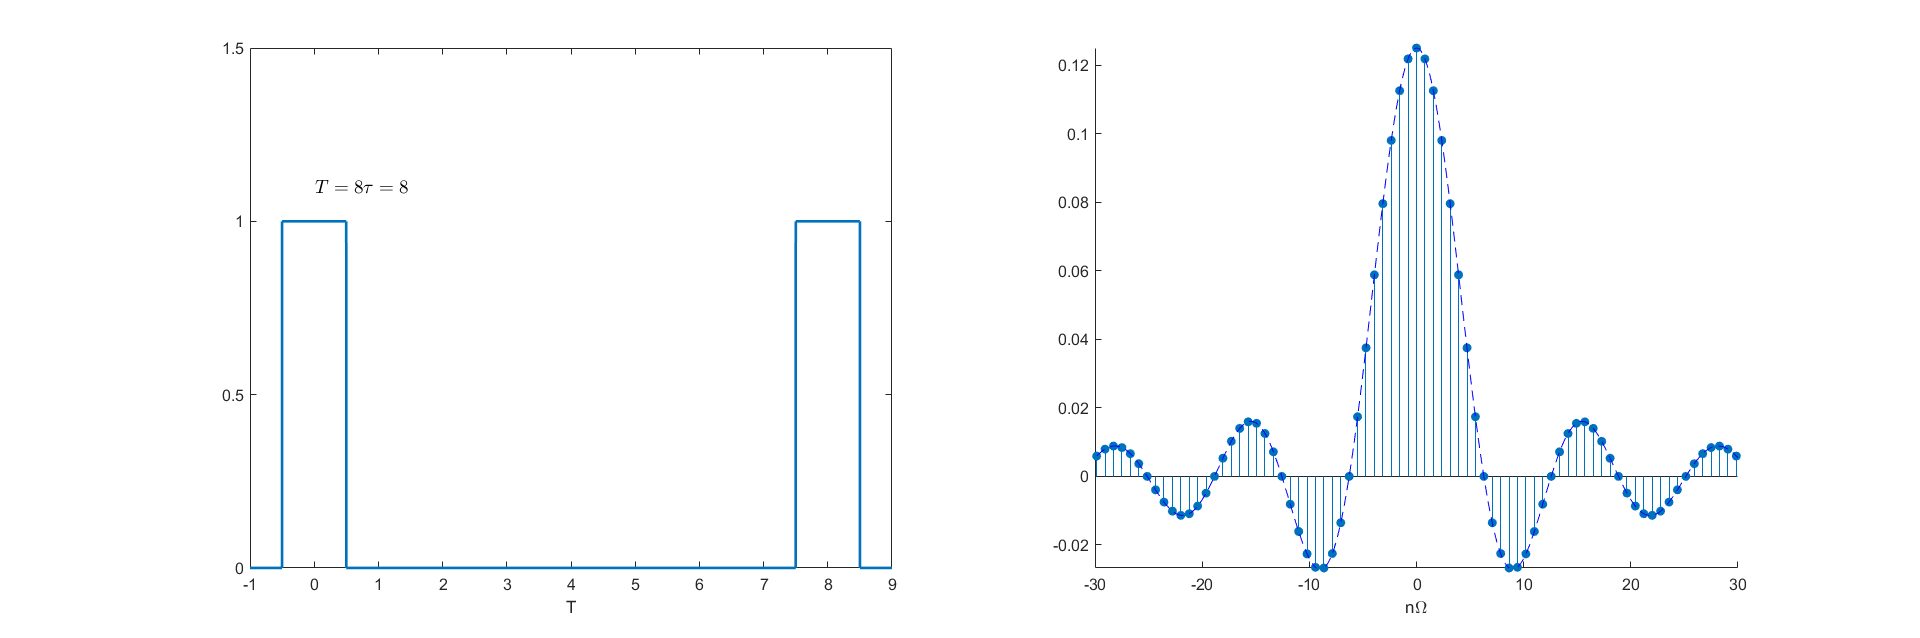
\includegraphics[width=0.9\linewidth]{figure/bw_5.png}}
	\centerline{\textbf{$T = 8\tau = 8$}}
\end{figure}
\begin{figure}[H]
	\centerline{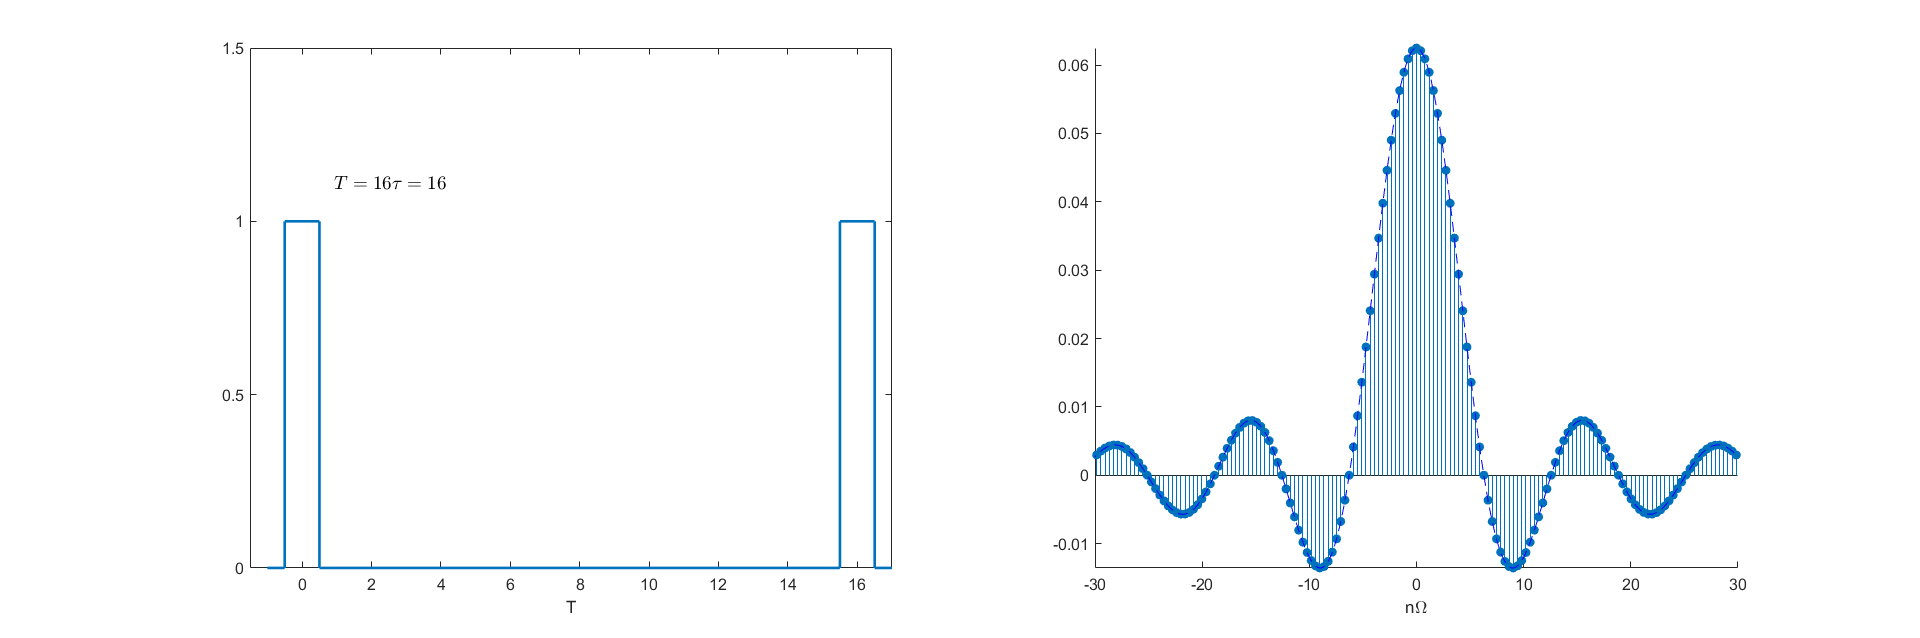
\includegraphics[width=0.9\linewidth]{figure/bw_6.png}}
	\centerline{\textbf{$T = 16\tau = 16$}}
\end{figure}
And through these three figures, we can obtain two other conclusions:
\begin{itemize}
	\item \textbf{Invariant $T$ and decreasing $\tau$:} The gap remains unchanged while signal bandwidth increases.
	\item \textbf{Invariant $\tau$ and increasing $T$:} The gap shrinks while signal bandwidth not change.
\end{itemize}
At this time, we will have a question, if $T$ tends to infinity, what will happen in the frequency domain. If $T\rightarrow \infty$, the signal will change from periodic to aperiodic. We can boldly assume that when the time-domain is aperiodic, the frequency-domain will become continuous. And let's prove it.
\clearpage

\section{\sc IV. From periodicity to aperiodicity}
\subsection{\sc \textbf{Just $T \rightarrow \infty$?}}
We can assume that the signal is defined over $[a,b]$. And the period of this signal is big enough to contain the whole signal. And we can calculate the Fourier series over the big period and making $T$ go to infinity.
\begin{align}
	C_n &= \frac{1}{T} \int_{-\frac{T}{2}}^{\frac{T}{2}} f(t) e^{-jn\Omega t} \dif t \nonumber \\ 
		&= \frac{1}{T} \int_{a}^{b} f(t) e^{-j \frac{2\pi n}{T} t} \dif t \nonumber
\end{align} 
The magnitude of $C_n$ can be calculated as
\begin{align}
	\left| C_n \right| 
	&= \frac{1}{T} \left| \int_{a}^{b} f(t) e^{-j \frac{2\pi n}{T} t} \dif t \right| \nonumber \\
	&\leq \frac{1}{T} \int_{a}^{b} \left| f(t) \right| \left| e^{-j\frac{2\pi n}{T} t} \right| \dif t \nonumber \\
	\left| C_n \right| 
	& \leq \frac{1}{T} \int_{a}^{b} \left| f(t) \right| \dif t \nonumber
\end{align}
The $\int_{a}^{b} \left| f(t) \right| \dif t $ is a definite integration, we can denote it by $M$.
$$
\left| C_n \right| \leq \frac{1}{T} M
$$
Apply limits to both sides
$$
\lim_{T\rightarrow \infty} \left| C_n \right| \leq \lim_{T\rightarrow \infty} \frac{1}{T} M = 0
$$
\subsection{\sc \textbf{Real Substitution Method}}
All coefficients go to zero! And we can obtain they are killed by the $\frac{1}{T}$. Well, it seems like just let's T goes to infinity is infeasible. Let's go back to the beginning and see what role $T$ plays in forming a signal.
By Fourier Series, we can obtain
\begin{align}
	&f(t) = \sum\limits_{n=-\infty}^{\infty} C_n e^{jn \Omega t} \label{FTAA} \\
	&C_n = \frac{1}{T} \int_{-\frac{T}{2}}^{\frac{T}{2}} f_T(t) e^{-jn\Omega t} \dif t 
	\quad \left(\Omega = \frac{2\pi}{T}\right) \label{FTBB}
\end{align}
Substitute \eqref{FTBB} into \eqref{FTAA}
\begin{align}
	f(t) = \sum\limits_{n=-\infty}^{\infty} 
		   \frac{1}{T} \left[ \int_{-\frac{T}{2}}^{\frac{T}{2}} f_T(t) e^{-jn\Omega t} \dif t \right]
		   e^{jn \Omega t} \nonumber
\end{align}
Let's denote $n\Omega = \omega$, we can get
\begin{align}
	 \Delta \omega &= (n+1)\Omega - n\Omega = \Omega = \frac{2\pi}{T} \label{FTCC} \\
	 f(t) 
	 &= \sum\limits_{n=-\infty}^{\infty} 
	 \frac{1}{T} \left[ \int_{-\frac{T}{2}}^{\frac{T}{2}} f_T(t) e^{-j\omega t} \dif t \right]
	 e^{j\omega t} \label{FTDD}
\end{align}
Substitute \eqref{FTCC} into \eqref{FTDD}
\begin{align}
	f(t) = \frac{1}{2\pi} \sum\limits_{n=-\infty}^{\infty} 
	\Delta \omega \left[ \int_{-\frac{T}{2}}^{\frac{T}{2}} f_T(t) e^{-j\omega t} \dif t \right]
	e^{j\omega t} \label{FTEE}
\end{align}
In \eqref{FTEE}, when $T \rightarrow \infty$, we can obtain
\begin{align}
	& \int_{-\frac{T}{2}}^{\frac{T}{2}} \rightarrow \int_{-\infty}^{\infty} \nonumber \\
	& \sum\limits_{n=-\infty}^{\infty} \Delta \omega \rightarrow \int_{-\infty}^{\infty} \dif \omega \nonumber \\
	& n\Omega \rightarrow \omega \nonumber
\end{align}
So, we can get
$$
f(t) = \frac{1}{2\pi} \int_{-\infty}^{\infty} e^{j\omega t} \dif \omega \int_{-\infty}^{\infty} f(t) e^{-j\omega t} \dif t
$$
So we can denote $\mathscr{F}_f(\omega) = \int_{-\infty}^{\infty} f(t) e^{-j\omega t} \dif t$. This is called the \textbf{Fourier Transform} of given signal $f(t)$.\par
Also we can get the \textbf{inverse Fourier Transform}:
$$
	f(t) = \frac{1}{2\pi} \int_{-\infty}^{\infty} \mathscr{F}_f(\omega) e^{j\omega t} \dif \omega
$$
The Fourier Transform of $f(t)$ exists if $f(t)$ is absolutely integrable.And $f(t)$ and $\mathscr{F}_f(\omega)$ together are defined as \textbf{Fourier Transform pair} as
$$
f(t) \stackrel{\mathscr{F}}{\longleftrightarrow} \mathscr{F}_f(\omega)
$$
\subsection{\sc \textbf{Fourier Transform of Common Functions}}
\begin{longtable}[c]{ccc}
	\caption{Fourier Transform of Common Function}
	\label{tab:my-table}\\
	\hline
	\endfirsthead
	%
	\endhead
	%
	No& \tabbox{$f(t)$} & \tabbox{$\ftfunc(\omega)$} \\ \hline
	1 & \tabbox{$e^{-at}$} & \tabbox{$\frac{1}{a+j\omega}$} \\
	2 & \tabbox{$e^{-a\left|t\right|}$} & \tabbox{$\frac{2a}{a^2+\omega^2}$} \\
	3 & \tabbox{$rect\left(\frac{t}{\tau}\right)$} & \tabbox{$\tau Sa(\frac{\omega\tau}{2})$} \\
	4 & \tabbox{$\delta(t)$} & \tabbox{$1$} \\
	5 & \tabbox{$sgn(t)$} & \tabbox{$\frac{2}{j\omega}$} \\
	6 & \tabbox{$u(t)$} & \tabbox{$\pi\delta(\omega)+\frac{1}{j\omega}$} \\
	7 & \tabbox{$cos(\omega_0 t)$} & \tabbox{$\pi\left[ \delta(\omega+\omega_0) + \delta(\omega-\omega_0) \right]$} \\
	8 & \tabbox{$sin(\omega_0 t)$} & \tabbox{$j\pi\left[ \delta(\omega+\omega_0) - \delta(\omega-\omega_0) \right]$} \\
	9 & \tabbox{$\frac{1}{t}$} & \tabbox{$-j\pi sgn(\omega)$} \\
	\hline
\end{longtable}
\clearpage
\subsection{\sc \textbf{Some Properties}}
% Please add the following required packages to your document preamble:
% \usepackage{longtable}
% Note: It may be necessary to compile the document several times to get a multi-page table to line up properly
\begin{longtable}[c]{ccc}
	\caption{Properties}
	\label{tab:my-table}\\
	\hline
	\endfirsthead
	%
	\endhead
	%
	\multicolumn{3}{l}{\tabbox{\textbf{Transformation}}} \\ \hline
	1 & Time-Domain Scaling & \tabbox{$ f(at) \ftarrow \frac{1}{\left| a \right|} \ftfunc(\frac{\omega}{a}) $} \\
	2 & Time-Domain Shifting & \tabbox{$ f(t-t_0) \ftarrow e^{-j\omega t_0} \ftfunc(\omega) $} \\
	3 & Frequency-Domain Shifting & \tabbox{$ f(t)e^{j\omega_0 t} \ftarrow \ftfunc(\omega-\omega_0) $} \\
	4 & Conjugate & \tabbox{$ f^*(t) \ftarrow \ftfunc^*(\omega) $} \\
	5 & Duality & \tabbox{$ \ftfunc(t) \ftarrow 2\pi f(-\omega) $} \\
	\hline
	\multicolumn{3}{l}{\tabbox{\textbf{Calculation}}} \\ \hline
	1 & Linearity & \tabbox{$ af_1(t)+bf_2(t) \ftarrow a\ftfunc_1(\omega)+b\ftfunc_2(\omega) $} \\
	2 & Time-Domain Convolution & \tabbox{$ f_1(t) \ast f_2(t) \ftarrow \ftfunc_1(\omega)\ftfunc_2(\omega) $} \\
	3 & Frequency-Domain Convolution & \tabbox{$ f_1(t)f_2(t) \ftarrow \frac{1}{2\pi}\ftfunc_1(\omega) \ast \ftfunc_2(\omega) $} \\
	4 & Time-Domain Differentiation & \tabbox{$ \frac{\dif^k}{\dif t^k}f(t) \ftarrow (j\omega)^k \ftfunc(\omega) $} \\
	5 & Time-Domain Integration & \tabbox{$ \int_{-\infty}^{t} f(\tau) \dif \tau \ftarrow \pi \ftfunc(0) \delta(\omega) + \frac{\ftfunc(\omega)}{j\omega} $} \\
	6 & Frequency-Domain Differentiation & \tabbox{$ t^kf(t) \ftarrow (j)^k\frac{\dif^k}{\dif \omega^k} \ftfunc(\omega) $} \\
	\hline
	\multicolumn{3}{l}{\tabbox{\textbf{Parseval's Theorem}}} \\ \hline
	\multicolumn{3}{c}{\tabbox{$\int_{-\infty}^{\infty} \left|f(t)\right|^2 \dif t = \frac{1}{2\pi} \int_{-\infty}^{\infty}\left|\mathscr{F}_f(\omega)\right|^2 \dif \omega$}} \\ \hline
\end{longtable}
\subsection{\sc \textbf{One Target Two World}}
\begin{figure}[H]
	\centering
	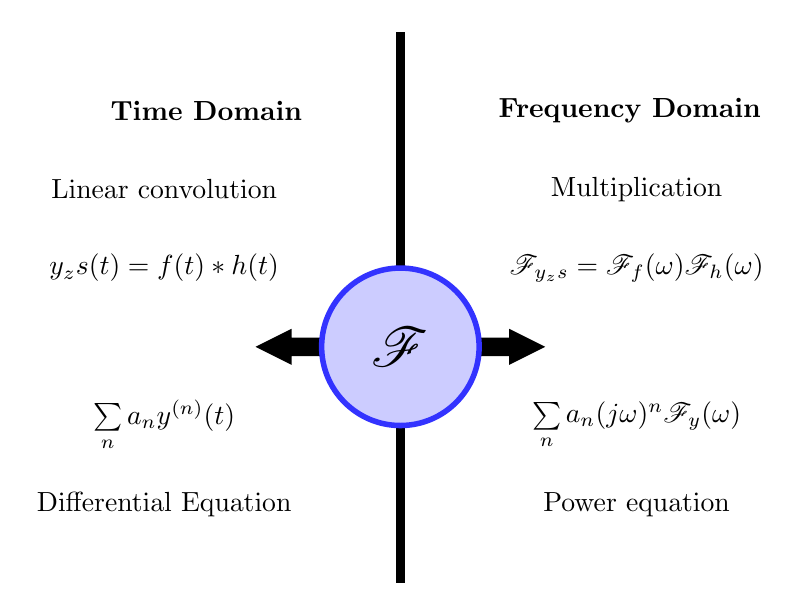
\begin{tikzpicture}
		\draw[line width=3pt] (0,1) -- (0,4);
		\draw[line width=3pt] (0,-1) -- (0,-3);
		\filldraw[line width=1pt,fill=black] (-0.9,0.1) -- (-1.4,0.1) -- (-1.4,0.2) -- (-1.8,0) -- (-1.4,-0.2) -- (-1.4,-0.1) -- (-0.9,-0.1) -- cycle;
		\filldraw[line width=1pt,fill=black] (0.9,0.1) -- (1.4,0.1) -- (1.4,0.2) -- (1.8,0) -- (1.4,-0.2) -- (1.4,-0.1) -- (0.9,-0.1) -- cycle;
		\filldraw[line width=2pt,draw=blue!80,fill=blue!20] (0,0) circle(1);
		\node[scale=2] (1) at (0,0) {$\mathscr{F}$};
		\node (2) at (-3,2) {Linear convolution};
		\node (3) at (-3,1) {$y_zs(t)=f(t) \ast h(t)$};
		\node (4) at (3,2) {Multiplication};
		\node (5) at (3,1) {$\mathscr{F}_{y_zs} = \mathscr{F}_f(\omega)\mathscr{F}_h(\omega) $};
		\node (6) at (-3,-2) {Differential Equation};
		\node (7) at (-3,-1) {$\sum\limits_n a_ny^{(n)}(t)$};
		\node (8) at (3,-2) {Power equation};
		\node (9) at (3,-1) {$\sum\limits_n a_n(j\omega)^n\mathscr{F}_y(\omega)$};
		\node (p) at (0,3) {};
		\node[left=of p] {\textbf{Time Domain}};
		\node[right=of p] {\textbf{Frequency Domain}};
	\end{tikzpicture}
\end{figure}
\clearpage

\end{resume}
\end{document}




